% -----------------------------*- LaTeX -*------------------------------
\documentclass[UTF8]{report}
% ------------------------------------------------------------------------
% Packages
% ------------------------------------------------------------------------
\usepackage{ctex}
\usepackage[body={7in, 9in},left=1in,right=1in]{geometry}
\usepackage{amsmath,amsfonts,amssymb,bm,amsthm}%数学宏包、数学字体、数学符号、支持 \mathscr{} 字体、支持粗斜体 \bm{}、数学定理
\usepackage{graphicx}%支持 \includegraphics{} 插图
\usepackage{subfigure}%插入子图
\usepackage{nicefrac}
\usepackage{mathrsfs}
\usepackage{caption}
\usepackage{algorithm,algorithmicx}
\usepackage[noend]{algpseudocode}
\usepackage{fancyhdr}
\usepackage{adjustbox}
\usepackage{esint}%支持多种积分算子
\usepackage{mathtools}%数学宏包的重要补充
\usepackage{upgreek}%数学环境的直立希腊字母
\usepackage{enumitem}%自定义列表环境
\usepackage{color}%支持颜色改变
\usepackage{extarrows}%任意长度的箭头
\usepackage{tikz,xcolor}%画图、画 Feynman 图
\usepackage{breqn}
\usepackage{fontsize}
\usepackage[framemethod=TikZ]{mdframed}
\usepackage{fontspec}
\usepackage{bigstrut,multirow,rotating}%Excel表格自动导入latex
\usepackage{booktabs}
\usepackage{scribe}
% ------------------------------------------------------------------------
% Macros
% ------------------------------------------------------------------------
%~~~~~~~~~~~~~~~
% Utility latin
%~~~~~~~~~~~~~~~
\newcommand{\ie}{\textit{i.e.}}
\newcommand{\eg}{\textit{e.g.}}
%~~~~~~~~~~~~~~~
% Environment shortcuts
%~~~~~~~~~~~~~~~
\newcommand{\balign}[1]{\ealign{\begin{align}#1\end{align}}}
\newcommand{\baligns}[1]{\ealigns{\begin{align*}#1\end{align*}}}
\newcommand{\bitemize}[1]{\eitemize{\begin{itemize}#1\end{itemize}}}
\newcommand{\benumerate}[1]{\eenumerate{\begin{enumerate}#1\end{enumerate}}}
%~~~~~~~~~~~~~~~
% Text with quads around it
%~~~~~~~~~~~~~~~
\newcommand{\qtext}[1]{\quad\text{#1}\quad}
%~~~~~~~~~~~~~~~
% Shorthand for math formatting
%~~~~~~~~~~~~~~~
\newcommand{\mbb}[1]{\mathbb{#1}}
\newcommand{\mbi}[1]{\boldsymbol{#1}} % Bold and italic (math bold italic)
\newcommand{\mbf}[1]{\mathbf{#1}}
\newcommand{\mc}[1]{\mathcal{#1}}
\newcommand{\mrm}[1]{\mathrm{#1}}
\newcommand{\tbf}[1]{\textbf{#1}}
\newcommand{\tsc}[1]{\textsc{#1}}
%\def\\langle {{\langle }}
%\def\\rangle {{\rangle }}
\newcommand{\sT}{\sf T}
\newcommand{\grad}{\nabla}
\newcommand{\Proj}{\Pi}
%~~~~~~~~~~~~~~~
% Common sets 定义数集符号
%~~~~~~~~~~~~~~~
\newcommand{\R}{\mathbb{R}}
\newcommand{\Z}{\mathbb{Z}}
\newcommand{\Q}{\mathbb{Q}}
\newcommand{\N}{\mathbb{N}}
\newcommand{\C}{\mathbb{C}}
\newcommand{\reals}{\mathbb{R}} % Real number symbol
\newcommand{\integers}{\mathbb{Z}} % Integer symbol
\newcommand{\rationals}{\mathbb{Q}} % Rational numbers
\newcommand{\naturals}{\mathbb{N}} % Natural numbers
\newcommand{\complex}{\mathbb{C}} % Complex numbers
%~~~~~~~~~~~~~~~
% Common functions
%~~~~~~~~~~~~~~~
\renewcommand{\exp}[1]{\operatorname{exp}\left(#1\right)} % Exponential
\newcommand{\indic}[1]{\mbb{I}\left(#1\right)} % Indicator function
\newcommand{\indicsub}[2]{\mbb{I}_{#2}\left(#1\right)} % Indicator function
\newcommand{\argmax}{\mathop\mathrm{arg\, max}} % Defining math symbols
\newcommand{\argmin}{\mathop\mathrm{arg\, min}}
\renewcommand{\arccos}{\mathop\mathrm{arccos}}
\newcommand{\dom}{\mathop\mathrm{dom}} % Domain
\newcommand{\range}{\mathop\mathrm{range}} % Range
\newcommand{\diag}{\mathop\mathrm{diag}}
\newcommand{\tr}{\mathop\mathrm{tr}}
\newcommand{\abs}{\mathop\mathrm{abs}}
\newcommand{\card}{\mathop\mathrm{card}}
\newcommand{\sign}{\mathop\mathrm{sign}}
\newcommand{\prox}{\mathrm{prox}} % prox
\newcommand{\rank}[1]{\mathrm{rank}(#1)}
\newcommand{\supp}[1]{\mathrm{supp}(#1)}
\newcommand{\norm}[1]{\lVert#1\rVert}
%~~~~~~~~~~~~~~~
% Common probability symbols
%~~~~~~~~~~~~~~~
\newcommand{\family}{\mathcal{P}} % probability family / statistical model
\newcommand{\iid}{\stackrel{\mathrm{iid}}{\sim}}
\newcommand{\ind}{\stackrel{\mathrm{ind}}{\sim}}
\newcommand{\E}{\mathbb{E}} % Expectation symbol
\newcommand{\Earg}[1]{\E\left[#1\right]}
\newcommand{\Esubarg}[2]{\E_{#1}\left[#2\right]}
\renewcommand{\P}{\mathbb{P}} % Probability symbol
\newcommand{\Parg}[1]{\P\left(#1\right)}
\newcommand{\Psubarg}[2]{\P_{#1}\left[#2\right]}
%\newcommand{\Cov}{\mrm{Cov}} % Covariance symbol
%\newcommand{\Covarg}[1]{\Cov\left[#1\right]}
%\newcommand{\Covsubarg}[2]{\Cov_{#1}\left[#2\right]}
%\newcommand{\model}{\mathcal{P}} % probability family / statistical model
%~~~~~~~~~~~~~~~
% Distributions
%~~~~~~~~~~~~~~~
%\newcommand{\Gsn}{\mathcal{N}}
%\newcommand{\Ber}{\textnormal{Ber}}
%\newcommand{\Bin}{\textnormal{Bin}}
%\newcommand{\Unif}{\textnormal{Unif}}
%\newcommand{\Mult}{\textnormal{Mult}}
%\newcommand{\NegMult}{\textnormal{NegMult}}
%\newcommand{\Dir}{\textnormal{Dir}}
%\newcommand{\Bet}{\textnormal{Beta}}
%\newcommand{\Gam}{\textnormal{Gamma}}
%\newcommand{\Poi}{\textnormal{Poi}}
%\newcommand{\HypGeo}{\textnormal{HypGeo}}
%\newcommand{\GEM}{\textnormal{GEM}}
%\newcommand{\BP}{\textnormal{BP}}
%\newcommand{\DP}{\textnormal{DP}}
%\newcommand{\BeP}{\textnormal{BeP}}
%\newcommand{\Exp}{\textnormal{Exp}}
%~~~~~~~~~~~~~~~
% Theorem-like environments
%~~~~~~~~~~~~~~~
%\theoremstyle{definition}
%\newtheorem{definition}{Definition}
%\newtheorem{example}{Example}
%\newtheorem{problem}{Problem}
%\newtheorem{lemma}{Lemma}
%~~~~~~~~~~~~~~~
% 组合数学的模板和作业里用到的一些宏包和自定义命令
%~~~~~~~~~~~~~~~
\renewcommand{\emph}[1]{\begin{kaishu}#1\end{kaishu}}
\newcommand{\falfac}[1]{^{\underline{#1}}}
\newcommand{\binomfrac}[2]{\frac{#1^{\underline{#2}}}{#2!}}
\newcommand{\ceil}[1]{\left\lceil #1 \right\rceil}
\newcommand{\floor}[1]{\left\lfloor #1 \right\rfloor}
\newcommand{\suminfty}[2]{\sum_{#1=#2}^{\infty}}
\newcommand{\suminftyk}[0]{\sum_{k=0}^{\infty}}
\newcommand{\sumint}[3]{\sum_{#1=#2}^{#3}}
\newcommand{\sumintk}[2]{\sum_{k=#1}^{#2}}
\newcommand{\suminti}[2]{\sum_{i=#1}^{#2}}
%~~~~~~~~~~~~~~~
% 定义新命令
%~~~~~~~~~~~~~~~
\newcommand*{\unit}[1]{\mathop{}\!\mathrm{#1}}
\newcommand*{\dif}{\mathop{}\!\mathrm{d}}%微分算子 d
\newcommand*{\pdif}{\mathop{}\!\partial}%偏微分算子
\newcommand*{\cdif}{\mathop{}\!\nabla}%协变导数、nabla 算子
\newcommand*{\laplace}{\mathop{}\!\Delta}%laplace 算子
\newcommand*{\deriv}[2]{\frac{\mathrm{d} #1}{\mathrm{d} {#2}}}
\newcommand*{\derivh}[3]{\frac{\mathrm{d}^{#1} #2}{\mathrm{d} {#3^{#1}}}}
\newcommand*{\pderiv}[2]{\frac{\partial #1}{\partial {#2}}}
\newcommand*{\pderivh}[3]{\frac{\partial^{#1} #2}{\partial {#3^{#1}}}}
\newcommand*{\dderiv}[2]{\dfrac{\mathrm{d} #1}{\mathrm{d} {#2}}}
\newcommand*{\dderivh}[3]{\dfrac{\mathrm{d}^{#1} #2}{\mathrm{d} {#3^{#1}}}}
\newcommand*{\dpderiv}[2]{\dfrac{\partial #1}{\partial {#2}}}
\newcommand*{\dpderivh}[3]{\dfrac{\partial^{#1} #2}{\partial {#3^{#1}}}}
\newcommand{\me}[1]{\mathrm{e}^{#1}}%e 指数
\newcommand{\mi}{\mathrm{i}}%虚数单位
%\newcommand{\mc}{\mathrm{c}}%光速 定义与mathcal冲突
\newcommand{\red}[1]{\textcolor{red}{#1}}
\newcommand{\blue}[1]{\textcolor{blue}{#1}}
%\newcommand{\Rome}[1]{\setcounter{rome}{#1}\Roman{rome}}
%~~~~~~~~~~~~~~~
% 公式环境中箭头符号的简写
%~~~~~~~~~~~~~~~
\newcommand{\ra}{\rightarrow}
\newcommand{\Ra}{\Rightarrow}
\newcommand{\la}{\leftarrow}
\newcommand{\La}{\Leftarrow}
\newcommand{\lra}{\leftrightarrow}
\newcommand{\Lra}{\Leftrightarrow}
\newcommand{\lgla}{\longleftarrow}
\newcommand{\Lgla}{\Longleftarrow}
\newcommand{\lgra}{\longrightarrow}
\newcommand{\Lgra}{\Longrightarrow}
\newcommand{\lglra}{\longleftrightarrow}
\newcommand{\Lglra}{\Longleftrightarrow}
%~~~~~~~~~~~~~~~
% 一些数学的环境设置
%~~~~~~~~~~~~~~~
%\newcounter{counter_exm}\setcounter{counter_exm}{1}
%\newcounter{counter_prb}\setcounter{counter_prb}{1}
%\newcounter{counter_thm}\setcounter{counter_thm}{1}
%\newcounter{counter_lma}\setcounter{counter_lma}{1}
%\newcounter{counter_dft}\setcounter{counter_dft}{1}
%\newcounter{counter_clm}\setcounter{counter_clm}{1}
%\newcounter{counter_cly}\setcounter{counter_cly}{1}
%\newtheorem{theorem}{{\hskip 1.7em \bf 定理}}
%\newtheorem{lemma}[theorem]{\hskip 1.7em 引理}
%\newtheorem{proposition}[theorem]{Proposition}
%\newtheorem{claim}[theorem]{\hskip 1.7em 命题}
%\newtheorem{corollary}[theorem]{\hskip 1.7em 推论}
%\newtheorem{definition}[theorem]{\hskip 1.7em 定义}
\newcommand{\problem}[1]{{\setlength{\parskip}{10pt}\noindent \bf{#1}}}
\newenvironment{solution}{{\noindent\hskip 2em \bf 解 \quad}}{}
\renewenvironment{proof}{{\setlength{\parskip}{7pt}\noindent\hskip 2em \bf 证明 \quad}}{\hfill$\qed$\par}
%\newenvironment{example}{{\noindent\hskip 2em \bf 例 \arabic{counter_exm}\quad}}{\addtocounter{counter_exm}{1}\par}
%\newenvironment{concept}[1]{{\bf #1\quad} \begin{kaishu}} {\end{kaishu}\par}
%~~~~~~~~~~~~~~~
% 本.tex文档中特殊定义命令
%~~~~~~~~~~~~~~~
\newcommand{\lno}[1]{\overline{#1}}
\newcommand{\NP}{\mathrm{NP}}
\newcommand{\ISO}{\mathrm{ISO}}
\newcommand{\SAT}{\mathrm{SAT}}
\newcommand{\threeSAT}{\mathrm{3\text{-}SAT}}
\renewcommand{\P}{\mathrm{P}}
\mathchardef\mhyphen="2D
\newcommand{\CNF}{\mathrm{CNF}}
\newcommand{\DNF}{\mathrm{DNF}}
\newcommand{\SetSp}{\mathrm{SET\text{-}SPLITTING}}
\newcommand{\PUZZLE}{\mathrm{PUZZLE}}
\newcommand{\SPATH}{\mathrm{SPATH}}
\newcommand{\LPATH}{\mathrm{LPATH}}
\newcommand{\UHAMPATH}{\mathrm{UHAMPATH}}

% ----------------------------------------------------------------------
% Header information
% ------------------------------------------------------------------------

\begin{document}

\course{B0911005Y-01} 			%optional
\coursetitle{Introduction to Theory of Computation}	%optional
\semester{2023 Spring}		%optional
\lecturer{Mingji Xia}	%optional
\scribe{吉骏雄}		%required
\lecturenumber{7}			%required (must be a number)
\lecturedate{May 26}	%required (omit year)

\maketitle

% ----------------------------------------------------------------------
% Body of the document
% ------------------------------------------------------------------------


\textbf{第7.1次作业:7.1abef,7.2abef,7.4,7.6,7.8,7.10}

\problem{7.1} 下面各项是真是假?
\begin{enumerate}[label={(\alph*)}]
    \item $2n = \operatorname*{O}(n)$
    \item $n^2 = \operatorname*{O}(n)$
    \setcounter{enumi}{4}
    \item $3^n = 2^{\operatorname*{O}(n)}$
    \item $2^{2^n} = \operatorname*{O}(2^{2^n})$
\end{enumerate}

\begin{solution}
    \begin{enumerate}[label={(\alph*)}]
        \item 真
        \item 假
        \setcounter{enumi}{4}
        \item 真
        \item 真
    \end{enumerate}
\end{solution}

\problem{7.2} 下面各项是真是假?
\begin{enumerate}[label={(\alph*)}]
    \item $n = \operatorname*{o}(2n)$
    \item $2n = \operatorname*{o}(n^2)$
    \setcounter{enumi}{4}
    \item $n = \operatorname*{o}(\log n)$
    \item $1 = \operatorname*{o}(1/n)$
\end{enumerate}

\begin{solution}
    \begin{enumerate}[label={(\alph*)}]
        \item 假
        \item 真
        \setcounter{enumi}{4}
        \item 假
        \item 假
    \end{enumerate}
\end{solution}


\problem{7.4} 对于字符串$w=baba $和下面的文法CFG $G$, 试填写定理$7.14$中识别上下文无关语言的多项式时间算法中所描绘的表:
\begin{align*}
    &S \to RT        \\
    &R \to TR \mid a \\
    &T \to TR \mid b
\end{align*}

\begin{solution}
    表格如下:
    \begin{table}[htbp]
        \centering
        \begin{tabular}{r|c|c|c|c|}
        \multicolumn{1}{r}{} & \multicolumn{1}{c}{1} & \multicolumn{1}{c}{2} & \multicolumn{1}{c}{3} & \multicolumn{1}{c}{4} \bigstrut[b]\\
        \cline{2-5} b $1$ & $T$ & $R\mid T$ & $S$ & $S\mid R\mid T$ \bigstrut\\
        \cline{2-5} a $2$ &     & $R$     & $S$   & $S$ \bigstrut\\
        \cline{2-5} b $3$ &     &         & $T$   & $R\mid T$ \bigstrut\\
        \cline{2-5} a $4$ &     &         &       & $R$ \bigstrut\\
        \cline{2-5}
        \end{tabular}%
    \end{table}%
    右上角有$S$, 所以可以生成串$w=baba$.
\end{solution}

\problem{7.6} 证明$P $在并、连接和补运算下封闭。

\begin{proof}
    并运算:

    $\forall L_1,L_2 \in P$, 根据定义, 存在两个图灵机$M_1,M_2$分别能够判定$L_1,L_2$, 且所需时间$f_1(n), f_2(n)$均为多项式时间. 我们构造一个图灵机$M'$:
    
    $M' =$ ``对于输入$\omega$, 其中$\omega$是字符串:
    \begin{enumerate}
        \item 将输入复制一份在带上输入右面, 左面的原输入暂时封存, 用不会出现在$M_1, M_2$带字符表的符号将之分隔开.
        \item 使用右侧复制的内容, 模拟在输入$\omega$上运行$M_1$.
        \item 如果$M_1$接受, 则接受; 如果$M_1$拒绝, 则清空分隔符右侧的内容, 返回原输入状态.
        \item 模拟在输入$\omega$上运行$M_2$.
        \item 如果$M_2$接受, 则接受; 如果$M_2$拒绝, 则拒绝.
        ''
    \end{enumerate}

    可以看到, $M'$的每一步都是多项式时间的, 且多步顺序执行. $M'$能判定$L_1\cup L_2$, 因此$L_1\cup L_2 \in P$. 因此$P$在并运算下封闭.

    连接运算:

    假设同上. 我们构造一个图灵机$M'$:
    
    $M' =$ ``对于输入$\omega$, 其中$\omega$是字符串:
    \begin{enumerate}
        \item 将输入复制一份在带上输入右面, 左面的原输入暂时封存, 用不会出现在$M_1, M_2$带字符表的符号将之分隔开.
        \item 遍历每一种将$\omega$分为两个前后连接的字符串$\omega_1, \omega_2$的可能性. 在每一种可能性中, 使用另一个不会出现在$M_1, M_2$带字符表的符号将之分隔开. 此时带上最后的字符串为$\omega_2$.
        \item 模拟在输入$\omega_2$上运行$M_2$.
        \item 如果$M_2$接受, 则清空$\omega_2$, 继续下一步; 如果$M_2$拒绝, 则恢复输入, 开启下一步循环.
        \item 模拟在输入$\omega_1$上运行$M_1$.
        \item 如果$M_2$接受, 则接受; 如果$M_2$拒绝, 则恢复输入, 开启下一步循环.
        ''
    \end{enumerate}

    可以看到, $M'$的每一步都是多项式时间的, 且循环最多进行$n+1$次, 复杂多也是多项式级别的 (因为是$n\cdot \operatorname{O}(f_1(n) + f_2(n) + p(n))$, 其中$p(n)$为一个多项式, 是其他步骤计算花费的时间). $M'$能判定$L_1 L_2$, 因此$L_1L_2 \in P$. 因此$P$在连接运算下封闭.

    补运算:

    $\forall L \in P$, 根据定义, 存在图灵机$M$能够判定$L$, 且所需时间$f$为多项式时间. 我们构造一个图灵机$M'$, 其与$M$的区别仅为接受状态与拒绝状态互换, 即$q_{\mathrm{accept}}$与$q_{\mathrm{reject}}$互换. 这样构造的图灵机依然可以对任意输入停机, 所需的计算时间一致, 且接受的语言恰为$\overline{L}$. 因此$P$在补运算下封闭.
\end{proof}

\problem{7.8} 令$\operatorname*{CONNECTED} = \{\langle G \rangle \mid G \text{是连通的无向图}\}$。分析3.3.2节给出的算法,证明此语言属千$P$。

\begin{proof}
    书中给出一种图灵机的构造:
    
    $M =$ ``输入是图$G$的编码$\langle G \rangle$:
    \begin{enumerate}
        \item 选择$G $的第一个顶点,并标记之。
        \item 重复下列步骤,直到没有新的顶点可作标记。
        \item 对于$G $的每一个顶点,如果能通过一条边将其连到另一个已被标记的顶点,则标记该顶点。
        \item 扫描$G $的所有顶点,确定它们是否都已作了标记。如果是,则接受,否则拒绝。
        ''
    \end{enumerate}
    
    在此构造中, 我们不难发现, 循环不超过$n$次 (因为字符串长度肯定超过图的顶点个数); 每次循环即便检查其他所有边, 也不会检查超过$n$次 (边数同样小于字符串长度); 最多标记$n$个顶点, 每标记一次顶点, 肯定在多项式时间内能够解决 (譬如将剩余字符串后移, 在顶点后添加固定长度标记, 这样的复杂度是$\operatorname*{O}(n)$); 而且这个图灵机可以停机. 综合来看, 这个图灵机总是能在多项式时间内完成判定. 所以此语言属千$P$.
\end{proof}

\problem{7.10} 证明$ALL_{DFA} \in P$.

\begin{proof}
    构造图灵机$M$判定$ALL_{DFA}$, 如下:

    $M' =$ ``对于输入$\langle A \rangle$, 其中$\langle A \rangle$应当是DFA的编码:
    \begin{enumerate}
        \item 判断$A$是否是一台DFA, 如果不是则拒绝.
        \item 寻找$A$中是否有拒绝状态$q_{reject}$. 如果没有, 则接受; 如果有, 重复下一步骤,直到没有新的顶点可作标记.
        \item 对于$A$的每一个状态, 如果能转换到另一个已被标记的状态, 则标记该状态.
        \item 检查$A$的初始状态$q_{0}$, 确定它是否已作了标记. 如果是, 则拒绝, 否则接受.
        ''
    \end{enumerate}

    因为一台$DFA$只要有能够从初始状态进入的拒绝状态, 那么一定会对某些字符串拒绝, 因此这台图灵机能够判定语言$ALL_{DFA}$
\end{proof}

\newpage

\textbf{第7.2次作业:7.5,7.7,7.12,7.35. 选做:7.13(较难),7.42}

\problem{7.5} 下面的公式是可满足的吗?
\[
    (x \lor y) \land (x \lor \lno y) \land (\lno x \lor y) \land (\lno x \lor \lno y)
\]

\begin{solution}
    不是. 化简:
    \begin{align*}
         {}& (x \lor y) \land (x \lor \lno y) \land (\lno x \lor y) \land (\lno x \lor \lno y) \\
        ={}& [(x \lor y) \land (x \lor \lno y)] \land [(\lno x \lor y) \land (\lno x \lor \lno y)] \\
        ={}& x \land \lno x \\
        ={}& 0
    \end{align*}
    因此不可满足.
\end{solution}

\problem{7.7} 证明$\NP$在并和连接运算下封闭。

\begin{proof}
    给出两种识别非确定型图灵机的构造如下: 
    \begin{enumerate}[label=(\arabic*)]
        \item 并运算:
        任意给定两个语言$A, B \in \NP$, 那么存在两个非确定型图灵机$M_1, M_2$能够在多项式时间内判定$A, B$. 我们构造一个非确定型图灵机$M'$:
        ``对于输入$\omega$, 其中$\omega$是字符串:
        \begin{enumerate}
            \item 以$\omega$为输入, 模拟运行$M_1$. 如果接受, 则继续下一步; 如果拒绝, 则拒绝.
            \item 以$\omega$为输入, 模拟运行$M_2$. 如果接受, 则接受; 如果拒绝, 则拒绝.
        \end{enumerate}
        ''

        \item 连接运算:
        任意给定两个语言$A, B \in \NP$, 那么存在两个非确定型图灵机$M_1, M_2$能够在多项式时间内判定$A, B$. 我们构造一个非确定型图灵机$M'$:
        ``对于输入$\omega$, 其中$\omega$是字符串:
        \begin{enumerate}
            \item 将原输入封存, 用不会出现在$M_1, M_2$带字符表的符号 (以\#为例) 做标记.
            \item 在原输入的最末端添加一个不会出现在$M_1, M_2$带字符表的符号 (以*为例) 做标记.
            \item 重复下2个步骤, 直到无法继续:
            \item 将*左侧的原始输入复制到右侧, 作为新的输入, 模拟运行$M_1$. 若接受, 则继续下一步; 若拒绝, 则继续回到第2步.
            \item 将*右侧的原始输入复制到左侧, 作为新的输入, 模拟运行$M_2$. 若接受, 则接受; 若拒绝, 则继续回到第2步.
            \item 若*抵达原输入$\omega$的最左侧, 即便使用空串运行$M_1$也不能接受, 则拒绝.
        \end{enumerate}
        ''
        由于中间的重复/计算都是多项式时间内可计算的, 于是这两个新的非确定型图灵机也是多项式时间内可计算的. 因此$\NP$在并和连接运算下封闭.
    \end{enumerate}
\end{proof}


\problem{7.12} 若图$G$的结点重新排序后,$G$可以变得与$H$完全相同,则称$G$与$H $是同构的 (isomorphic) 。令$\ISO = \{ \langle G, H \rangle \mid G \text{ 和 } H \text{ 是同构的图 }\}$。证明$\ISO \in \NP$.

\begin{proof}
    任意给定两个图$G, H$, 我们构造一个非确定型图灵机$M$:
    ``对于输入$\langle G, H \rangle$, 其中$G, H$是图的编码:
    \begin{enumerate}
        \item 检查$G, H$的结点数, 边数是否相同. 如果不同, 则拒绝.
        \item 对每一个$G$的结点$v$, 非确定地选择一个$H$的结点$w$, 并记录. 这共要进行$n$次选择, 其中$n$是$G$的结点数.
        \item 对每一对选中的结点$v, w$, 检查$G$中$v$的邻接结点是否与$H$中$w$的邻接结点相同, 即它们对其他每一对结点, 是否同时有/没有边分别与之相连. 这对每对结点来说, 共要进行$n$次检查, 其中$n$是$G$的结点数. 如果相同, 则接受. 如果不同, 则拒绝.
        ''
    \end{enumerate}
    ''

    这个非确定型图灵机的多项式时间性质是显然的, 因为共需要进行$n + n^2$次多项式时间内即可完成的可计算操作, 且$n < |\langle G, H \rangle|$. 于是$\ISO \in \NP$.
\end{proof}


\problem{7.35} 证明:若$\P=\NP$, 则任给布尔公式$\phi$,若$\phi$是可满足的,则存在多项式时间算法给出一个$\phi$的满足赋值。

(注意:要求提供的算法计算一个函数而非若干函数,除非是$\NP$包含的语言。$\P = \NP$的假定说明$\SAT$在$\P$中,所以其可满足性的验证是多项式时间可解的。但是这个假设没有说明这项验证如何进行,而且验证不能给出满足赋值。必须证明它们一定能够被找到。提示:重复地使用可满足性验证器一位一位地找出满足赋值。)

\begin{proof}
    任意给定一个布尔公式$\phi$, 我们构造一个非确定型图灵机$M$:
    ``对于输入$\phi$, 其中$\phi$是布尔公式:
    \begin{enumerate}
        \item 列出$\phi$中的所有变量.
        \item 非确定地对$\phi$中的每一个变量进行赋值, 并记录. 这共要进行$n$次选择, 每次选择在$0,1$中进行, 其中$n$是$\phi$的变量数.
        \item 调用$\SAT$的验证器, 验证$\phi$在这组赋值下是否可满足. 如果是, 则接受. 如果不是, 则拒绝.
    \end{enumerate}
    ''

    列出变量显然是多项式时间内可解的. 非确定地对每一个变量进行赋值, 也是多项式时间内可解的, 因为任意一条计算分支只需要赋值$n$次, 且$n < |\langle \phi\rangle|$, 每次赋值的时间是多项式的. 调用$\SAT$的验证器也只需要多项式时间, 因为$\P = \NP$且$\SAT \in \NP$, 因此$\SAT \in \P$. 因此这个非确定型图灵机的多项式时间性质是显然的. 于是$\SAT \in \NP$.
\end{proof}

\newpage

\textbf{第7.3次作业:7.29,7.39,7.45,7.48. 选做:7.38.}

\problem{7.29} 令$\SetSp = \{ \langle S,C \rangle \mid S \text{是一个有穷集, } C= \{ C_1, \dots , C_k\} \text{是由} S \text{的某些子集组成的集合, } k>0, \text{使得}S\text{的元素可以被染为红色或蓝色,而且对所有} C_i, C_i\text{中的元素不会被染成同一种颜色} \}$。

证明$\SetSp$是$\NP$完全的。

\begin{proof}
    \begin{enumerate}
        \item
        首先, 可以证明是$\SetSp \in \NP$. 给定一个$\langle S,C \rangle$, 我们构造一个非确定型图灵机$M$:
        ``对于输入$\langle S,C \rangle$, 其中$S$是一个有穷集, $C= \{ C_1, \dots , C_k\}$是由$S$的某些子集组成的集合, $k>0$:
        \begin{enumerate}
            \item 非确定地对$S$中的每一个元素进行染色, 并记录. 这共要进行$|S|$次选择, 每次选择在红/蓝中进行.
            \item 对于每一个$C_i,\ i\in \{1,\dots,k\}$, 验证 $C_i$中的元素不会被染成同一种颜色. 如果不是, 则拒绝.
            \item 如果均不会被染成同一种颜色, 则接受.
        \end{enumerate}
        ''

        在这个构造中, 我们显然仅使用了多项式时间就能完成问题的解决. 因此$\SetSp \in \NP$.

        \item
        通过证明$\threeSAT \leq_p \SetSp$来证明$\SetSp$是$\NP$完全的. 构造一个图灵机$M$: ``对于输入$\phi$, 其中$\phi$是$3\CNF$-布尔公式:
        \begin{enumerate}
            \item 列出$\phi$中的所有变量, 构成集合$V$.
            \item 构建集合$V' = \{a_i \mid a \in V,\ i\ \in \{0,1\}\}$
            \item 构造集合$S = V' \cup \{s\}$, 其中$s \notin V \cup V'$是一个新的变量.
            \item 再构造集合$A = \{\{a_i,b_j,c_k, s\} \mid a_i,b_j,c_k \in V';\ \forall x \in V, \text{ 我们取 }x_0 = x, x_1=\lno x,$ 且在这种赋值下 ,$\ \phi \text{ 中存在一个子句, 形如 } a_i \lor b_j \lor c_k \}$, 以及集合 $ B = \{ \{a_0, a_1\} \mid a \in V \}$. 取 $C = A \cup B$.
            \item 以$\langle S,C \rangle$为输入, 模拟运行$\SetSp$. 若接受, 则接受; 若拒绝, 则拒绝.
        \end{enumerate}
        ''
        
        第5步会得到$S$中是否存在满足条件的一种染色, 能让$C$中所有元素 (每个元素都是一个$S$的子集), 其内的元素 (也就是$S$中的一些元素) 获得的染色均不同. $A$中集合染色不同, 说明至少有一个元素与$s$的颜色不同; $B$中染色不同, 说明$a_0, a_1$的颜色不同. 这样, 我们不妨以与$s$ (s表示standard)颜色不同作为某个变量的赋值为$1/0$的标志: 若$a_1$与$s$颜色不同, 即$a_0$与$s$颜色相同, 这代表了$a$被赋值为$1$; 若$a_1$与$s$颜色相同, 即$a_0$与$s$颜色不同, 这代表了$a$被赋值为$0$. 根据这样的意义表示, $A$限制$\phi$的每一个子句都是可满足 (存在一个为$1$的文字), $B$要求了$\phi$的每一个变量的正确赋值.
        
        这样, 我们用$\SetSp$解决了$\threeSAT$, 这个归约成立. 并且很显然, 这个归约中的函数是多项式时间内即可计算的: 所有变量数少于输入字符串$|\langle\phi\rangle|$长度, 构造集合的难度也都在$O(|V|^3)$范围内. 因此, $\SetSp$是$\NP$完全的.
    \end{enumerate}
\end{proof}


\problem{7.39} 如图\ref{fig:7_39}, 有一个盒子和一些卡片,如下图所示。盒子里有栓塞,卡片上有凹口,所以每张卡片可以两种方式放入盒子中。每张卡片上有两排孔,有些孔没有打穿。把所有卡片放进盒子,使得盒子的底被完全覆盖 (即,每个孔的位置都被至少一张在该位置上无孔的卡片堵住),则谜题就算破解了。令$\PUZZLE = \{ \langle c_1, \dots ,c_k \rangle \mid \text{每个}c_i\text{代表一张卡片, 并且这个卡片集有解}\}$. 证明$\PUZZLE$是$\NP$完全的。
\begin{figure}[!htbp]
    \centering
    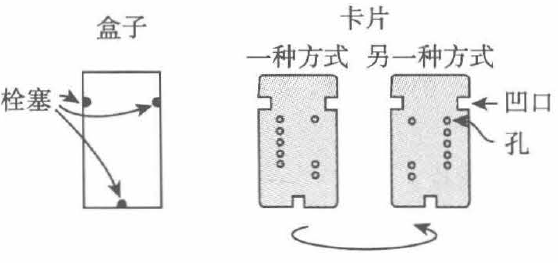
\includegraphics[width=7cm]{image/7.39.png}
    \caption{题7.39图}
    \label{fig:7_39}
\end{figure}

\begin{proof}
    \begin{enumerate}
        \item 
        首先, 可以证明是$\PUZZLE \in \NP$. 给定一个$\langle c_1, \dots ,c_k \rangle$, 我们构造一个非确定型图灵机$M$:
        ``对于输入$\langle c_1, \dots ,c_k \rangle$, 其中每个$c_i$代表一张卡片:
        \begin{enumerate}
            \item 非确定地对每一个卡片进行放置, 并记录. 这共要进行$k$次选择, 每次选择在两种放置方式 (对称的两种) 中进行. 
            \item 全部放好后, 检查盒子的底是否被完全覆盖. 如果是, 则接受. 如果不是, 则拒绝.
        \end{enumerate}
        ''

        这个方法中, 我们显然仅使用了多项式时间就能完成问题的解决. 因此$\PUZZLE \in \NP$.

        \item 
        再证明$\threeSAT \leq_p \PUZZLE$. 构造一个图灵机$M$: ``对于输入$\phi$, 其中$\phi$是$3\CNF$-布尔公式:
        \begin{enumerate}
            \item 列出$\phi$中的所有变量, 构成集合$V$, 并排序. 设$\phi$中有$n$个子句.
            \item 将$\lno\phi$转写为$3\DNF$的析取式, 比如$\phi = (x_1 \lor x_2 \lor \lno x_3) \land (\lno x_1 \lor x_2 \lor x_4)$, 则对应的$\lno \phi = \lno{(x_1 \lor x_2 \lor \lno x_3)} \lor \lno{(\lno x_1 \lor x_2 \lor x_4)} = (\lno x_1 \land \lno x_2 \land x_3) \lor (x_1 \land \lno x_2 \land \lno x_4)$
            \item 考虑$V$中的所有变量, 构成$|V|$张卡片, 第$i$张卡片的内容如下. 从上向下共有$n$对孔, 其中第$j$对孔, 代表$V$中第$i$个元素$v_i$在$\lno\phi$的第$j$个子句中的出现情况. 若未出现, 则有两个孔; 若出现$v_i$, 则左侧有一个孔; 若出现$\lno v_i$, 则右侧有一个孔 (合理地, 同时出现即可化简作未出现).
            
            例如, 若$\lno\phi = (\lno x_1 \land \lno x_2 \land x_3) \lor (x_1 \land \lno x_2 \land \lno x_4)$, 则:
            \begin{enumerate}
                \item 第1张卡片的内容为 ``自上而下, 第一处为右侧的孔, 第二处为左侧的孔'',
                \item 第2张卡片的内容为 ``自上而下, 第一处为右侧的孔, 第二处为右侧的孔'',
                \item 第3张卡片的内容为 ``自上而下, 第一处为左侧的孔, 第二处为一对孔'',
                \item 第4张卡片的内容为 ``自上而下, 第一处为一对孔, 第二处为右侧的孔''.
            \end{enumerate}
            这样的话, 如果四张卡片均正放, 就可以发现左侧一列两个孔洞均为封闭状态 (右侧我们并不关心). 这说明, 存在一组赋值使得$\lno\phi$的任意子句都是$0$ (以卡片开孔代表对应文字值为$1$, 孔洞位置开口对应子句值为$1$; 而封闭为$0$), 进而$\lno\phi = 0, \phi = 1$. 这样, 我们就证明了$\phi$是可满足的.

            \item 我们还需要检查左侧一列的所有洞是否都为封闭状态. 只要再加入一张卡牌$v_0$, 其左侧一列均为封闭, 右侧一列均开孔, 与之前的$|V|$张卡片一起形成卡片集合$\{v_0, v_1, \dots, v_k\}$. 由于对称性, 我们不妨认为$v_0$是正放的, 因为即便其反放, 我们也有一种相反的赋值方法, 使得问题存在一种对称的解. 
            \item 以$\langle v_0, v_1, \dots, v_k\rangle$作为输入, 模拟运行$\PUZZLE$. 若接受, 则接受; 若拒绝, 则拒绝.
        \end{enumerate}

        上文中的所有计算过程均为多项式时间可计算的. 因此, $\threeSAT \leq_p \PUZZLE$. 我们证明了$\PUZZLE$是$\NP$完全的.
    \end{enumerate}
\end{proof}





\problem{7.45} 证明若$\P = \NP$, 则除了语言$A = \varnothing$和$A = \Sigma^*$以外,所有语言$A \in \P$都是$\NP$完全的。

\begin{proof}
    首先, 显然, $\P \in \NP$. 所以除了语言$A = \varnothing$和$A = \Sigma^*$以外, 所有语言$A \in \P$都是属于$\NP$的.

    然后, 对于所有非平凡的语言$A \in \P$, 有$A \in \NP$根据题目假设. 那么根据定义, 对于任意语言$B \in \NP$, 都有$B \leq_p A$. 这件事其实很显然, 因为根据题目假设有$B \in \P$, 因此只需要用多项式时间计算出某个输入字符串$\omega$是否在$B$中, 然后将根据结果, 将一个是或不是在$A$中的串作为输入, 运行$A$本身, 就能调用$A$计算$B$. 构造图灵机如下:
    ``对于输入$\omega$, 其中$\omega$是字符串:
    \begin{enumerate}
        \item 事先准备好两个字符串$\omega_a, \omega_r$, 其中$\omega_a \in A, \omega_r \notin A$.
        \item 用多项式时间计算出$\omega$是否在$B$中. 如果是, 则以$\omega_a$作为下一问的输入; 如果不是, 则以$\omega_r$作为下一问的输入.
        \item 将上一问选定的字符串作为输入, 运行$A$. 如果接受, 则接受; 如果拒绝, 则拒绝.
    \end{enumerate}

    因此, $B \leq_p A$. 这说明, $A$是$\NP$完全的.
\end{proof}


\problem{7.48} 设$G $表示无向图,令
\[
    \SPATH = \{ \langle G,a,b,k \rangle \mid G \text{ 包含从 }a \text{ 到 }b \text{、长度至多为 }K \text{ 的简单路径 }\}
\]
以及
\[
    \LPATH = \{ \langle G,a,b,k \rangle \mid G \text{ 包含从 }a \text{ 到 }b \text{、长度至少为 }K \text{ 的简单路径 }\}
\]
\begin{enumerate}[label=\alph*.]
    \item 证明$\SPATH \in \P$。
    \item 证明$\LPATH$是$\NP$完全的。
\end{enumerate}

\begin{proof}
    \begin{enumerate}[label=\alph*.]
        \item 构造图灵机$M$能够识别$\SPATH$:
        ``对于输入$\langle G,a,b,k \rangle$, 其中$G$是无向图, $a,b$是$G$的两个顶点, $k$是一个正整数:
        \begin{enumerate}
            \item 从$a$开始, 以$1$为每条边的权重, 使用Dijkstra算法, 计算出从$a$到$b$的最短路径长度$d$. 如果$d \leq k$, 则接受; 如果$d > k$, 则拒绝.
        \end{enumerate}
        ''

        Dijkstra算法的时间复杂度是$\operatorname*{O}(n^2)$, 因此这个图灵机的多项式时间性质是显然的. 因此$\SPATH \in \P$.

        \item 首先证明$\LPATH \in \NP$. 构造非确定型图灵机$M$能够识别$\LPATH$:
        ``对于输入$\langle G,a,b,k \rangle$, 其中$G$是无向图, $a,b$是$G$的两个顶点, $k$是一个正整数:
        \begin{enumerate}
            \item 从$a$开始, 记录一条路径. 重复下一步骤$n - 1$次, 直到选到顶点$b$或没有任何相邻的顶点可选.
            \item 在路径最前方的顶点处, 非确定地确定其任意一个未被选进路径中的相邻顶点, 并将其加入路径中. 每次一共有至多$n-m$种选择, 其中$m$是路径中已有的顶点数. 将这个顶点视作路径最前方的结点.
            \item 如果选取到顶点$b$, 且得到的路径长度至少为$k$, 则接受; 否则, 则拒绝.
        \end{enumerate}
        ''

        这个非确定型图灵机的多项式时间性质是显然的. 因此$\LPATH \in \NP$.

        再来证明$\UHAMPATH \leq_p \LPATH$. 构造一个图灵机$M$: ``对于输入$\langle G, s, t \rangle$, 其中$G$是无向图, $s, t$是$G$的两个顶点:
        \begin{enumerate}
            \item $G=(V, E)$, 计算$|V| = n$为图$G$的顶点数.
            \item 以输入$\langle G, s, t, n-1 \rangle$, 运行$\LPATH$. 如果接受, 则接受; 如果拒绝, 则拒绝.
        \end{enumerate}
        ''

        很好理解, 因为$G$中的简单路径长度不可能超过$n-1$, 并且长度为$n-1$的路径一定是哈密顿路径. 很简单可以证明这个归约是多项式时间内可计算的, 因此$\LPATH$是$\NP$完全的.
    \end{enumerate}
\end{proof}


\end{document}
